% Generated figure: ../gen_v10/make_figures.py (fig_tradeoff) from out/qcore9_heldout/results.json (pooled_ABCD.rows: qcore6 on
% sets 1-3, qcore9 on set 4, hand identities). Values: ../gen_v10/figdata.json.
\begin{figure}[t]
\centering
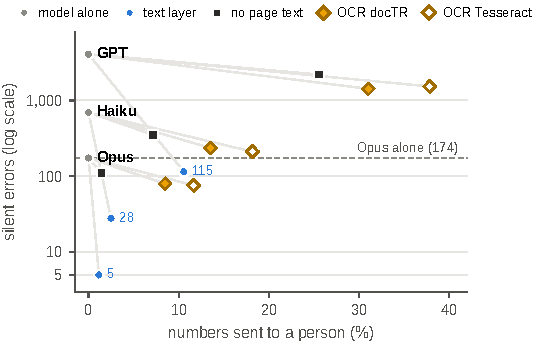
\includegraphics[width=\columnwidth]{v10_tradeoff.pdf}
\caption{Silent errors against the share of numbers sent to a person, SEC sets 1--4 pooled (17,125 numbers; hand identities, \vq{9} on set~4); thin lines join each model alone to its runs with the checker, and blue labels give the text-layer counts. Only the text layer takes the cheap model below Opus alone (dashed) at a small queue; OCR and no-text modes buy fewer silent errors with larger queues.}
\label{fig:tradeoff}
\end{figure}
